%**************************************************************************
%* SpringSim 2019 Author Kit
%*
%* Word Processing System: TeXnicCenter and MiKTeX
%*
%**************************************************************************
\documentclass{scspaperproc}

\usepackage{latexsym}
\usepackage{graphicx}
\usepackage{mathptmx}

%
%****************************************************************************
% AUTHOR: You may want to use some of these packages. (Optional)
%\usepackage{amsmath}
%\usepackage{amsfonts}
%\usepackage{amssymb}
%\usepackage{amsbsy}
%\usepackage{amsthm}
%****************************************************************************


%
%****************************************************************************
% AUTHOR: If you do not wish to use hyperlinks, then just comment
% out the hyperref usepackage commands below.

%% This version of the command is used if you use pdflatex. In this case you
%% cannot use ps or eps files for graphics, but pdf, jpeg, png etc are fine.

\usepackage[pdftex,colorlinks=true,urlcolor=blue,citecolor=black,anchorcolor=black,linkcolor=black]{hyperref}

%% The next versions of the hyperref command are used if you adopt the
%% outdated latex-dvips-ps2pdf route in generating your pdf file. In
%% this case you can use ps or eps files for graphics, but not pdf, jpeg, png etc.
%% However, the final pdf file should embed all fonts required which means that you have to use file
%% formats which can embed fonts. Please note that the final PDF file will not be generated on your computer!
%% If you are using WinEdt or PCTeX, then use the following. If you are using
%% Y&Y TeX then replace "dvips" with "dvipsone"

%% \usepackage[dvips,colorlinks=true,urlcolor=blue,citecolor=black,%
%% anchorcolor=black,linkcolor=black]{hyperref}

%% The use of the long citation format (e.g. "Brown and Edwards (1993)" rather than "[5]") and at the same
%% time using the hyperref package can lead to hard to trace bugs in case the citation is broken accross the
%% line (usually this will mark the entire paragraph as a hyperlink (clickable) which is easily noticeable and fixed
%% if using colorlinks, but not if the color is black -- as it is now). Worse yet, if a citation spans page boundary,
%% LaTeX compilation can fail, with an obscure error message. Since this depends a lot on the flow of the text
%% and wording, these bugs come and go and can be extremely hard for a beginner to trace. The error
%% message can look like this:
%%
%%    ! pdfTeX error (ext4): \pdfendlink ended up in different nesting level than \pdfstartlink.
%%    \AtBegShi@Output ...ipout \box \AtBeginShipoutBox 
%%    \fi \fi 
%%    l.174 
%%    ! ==> Fatal error occurred, no output PDF file produced!
%%
%% and can be universally fixed by putting an \mbox{} around the citation in question (in this case, at line 174)
%% and maybe adapting the wording a little bit to improve the paragraph typesetting, which is perhaps not
%% immediately obvious.
%****************************************************************************

%
%****************************************************************************
%*
%* AUTHOR: YOUR CALL!  Document-specific macros can come here.
%*
%****************************************************************************

\usepackage{float}
\usepackage{subcaption}
\usepackage{minted}
\usepackage{verbatim}
\usepackage[]{algorithm2e}

%#########################################################
%*
%*  The Document.
%*
\begin{document}

%***************************************************************************
% AUTHOR: AUTHOR NAMES GO HERE
% FORMAT AUTHORS NAMES Like: Author1, Author2 and Author3 (last names)
%
%		You need to change the author listing below!
%               Please list ALL authors using last name only, separate by a comma except
%               for the last author, separate with "and"
%
\SCSpagesetup{Thaler and Siebers}

% AUTHOR: Uncomment ONE of these correct conference names.
%\def\SCSconferenceacro{SpringSim}
\def\SCSconferenceacro{SummerSim}
%\def\SCSconferenceacro{AutumnSim}
%\def\SCSconferenceacro{PowerPlantSim}

% AUTHOR: Set the correct year of the conference.
\def\SCSpublicationyear{2019}

% AUTHOR: Set the correct month and dates; the dates are separated by a single minus sign
% with no spaces and no leading zeros, the month is a full name (e.g. April) with the first letter
% capitalized. For example, "April 8-13".
\def\SCSconferencedates{July 22-July 24}

% AUTHOR: Set the correct venue in the form "City, State, Country", for example "Los Angeles, CA, USA".
\def\SCSconferencevenue{Berlin, Germany}

% AUTHOR: Uncomment ONE of the track/symposium names where you are going to submit. Please, do NOT change.
% In case your symposium is not on this list, please DO contact your symposium chair.
%\def\SCSsymposiumacro{ANSS} % Annual Simulation Symposium
%\def\SCSsymposiumacro{CNS} % Communications and Networking Simulation Symposium
%\def\SCSsymposiumacro{HPC} % High Performance Computing Symposium
%\def\SCSsymposiumacro{TMS/DEVS} % Symposium on Theory of Modeling and Simulation
%\def\SCSsymposiumacro{ADS} % Agent-Directed Simulation
%\def\SCSsymposiumacro{MSCIAAS} % Modeling and Simulation of Complexity in Intelligent, Adaptive and Autonomous Systems
%\def\SCSsymposiumacro{MSM} % Modeling and Simulation in Medicine
%\def\SCSsymposiumacro{Mod4Sim} % Model-driven Approaches for Simulation Engineering Symposium
%\def\SCSsymposiumacro{Tutorial} % Tutorial Track
%\def\SCSsymposiumacro{WIP} % WIP Track
%\def\SCSsymposiumacro{Poster/Colloquium} % Poster Session and Student Colloquium
%\def\SCSsymposiumacro{MobileApp} % Student M\&S Mobile App Competition
%\def\SCSsymposiumacro{SPECTS} % Symposium on Performance Evaluation of Computer and Telecommunication Systems
\def\SCSsymposiumacro{SCSC} % Summer Computer Simulation Conference
%\def\SCSsymposiumacro{ICBGM} % International Conference on Bond-Graph Modeling
%\def\SCSsymposiumacro{Fossil} % Fossil Power Track
%\def\SCSsymposiumacro{Nuclear} % Nuclear Agent Power Track

% AUTHOR: Enter the title, all letters in upper case

\newminted[HaskellCode]{haskell}{fontsize=\footnotesize}

% Title portion. Note the short title for running heads
\title{THE AGENTS NEW CLOTHS? \\ \small{Towards Pure Functional Programming in ABS}}
%\subtitle{Towards Pure Functional Programming in ABS}

% AUTHOR: Enter the authors of the article, see end of the example document for further examples
\author{
\\%To level with the author block on the right.
Jonathan Thaler \\ 
Peer Olaf Siebers \\ [12pt] 
School Of Computer Science \\
University of Nottingham \\
%7301 Wollaton Rd \\
Nottingham, United Kingdom \\
\{jonathan.thaler,peer-olaf.siebers\}@nottingham.ac.uk\\
}

\maketitle

\section*{Abstract}
The established approach to implement and engineer Agent-Based Simulations (ABS) has primarily been object-oriented, with Python and Java being the most popular languages. In this paper we explore a different approach to this problem and investigate the pure functional programming paradigm, using the language Haskell. We give a high level introduction into the core features of pure functional programming and show how they can be made of use to implement ABS in a case-study of a full implementation of the seminal Sugarscape model. With this case-study we are able to show that pure functional programming as in Haskell has a valid place in building clean, robust and maintainable ABS implementations. Further we show that we can directly leverage the benefits of pure functional programming to ABS: we have strong guarantees of reproducibility at compile time, can easily exploit data-parallelism and concurrency is easier to get right. The main drawback is a lower performance than established performances but this was not the main focus of research and we hope to improve on this in the future.

\textbf{Keywords:} Agent-Based Simulation, Functional Programming.

\maketitle

\section{Introduction}
There exists a large number of simulation packages which allow the convenient creation of System Dynamics simulations by straight-forward visual diagram creation. One simply creates stocks and flows, connects them, specifies the flow-rates and initial parameters and then runs the model. An example for such a visual diagram creation in the simulation package AnyLogic can be seen in Figure \ref{fig:sir_stockflow_diagram}.

\begin{figure}
	\centering
	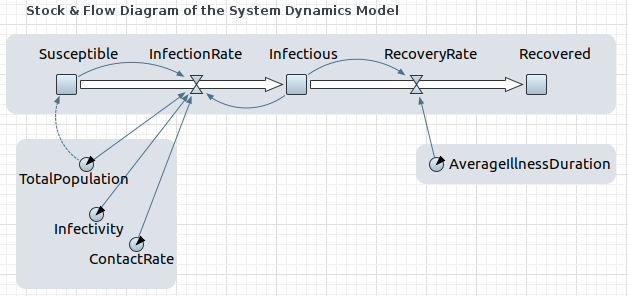
\includegraphics[width=.5\textwidth, angle=0]{./fig/SIR_SD_STOCKFLOW_DIAGRAMM.png}
	\caption{Visual System Dynamics Diagram of the SIR model in AnyLogic Personal Learning Edition 8.3.1.}
	\label{fig:sir_stockflow_diagram}
\end{figure}

Still, implementing System Dynamics directly in code is not as straight forward and involves numerical integration which can be quite tricky to get right. Thus, the aim of this paper is to look into how System Dynamics models can be implemented in code correctly without the use of a simulation package. We use the well known SIR model \cite{kermack_contribution_1927} from epidemiology to demonstrate our approach.

Our language of choice is Haskell because it emphasises a declarative programming style in which one describes \textit{what} instead of \textit{how} to compute. Further it allows to rule out interference with non-deterministic influences or side-effects already at compile-time. This is of fundamental importance for System Dynamics because it behaves completely deterministic and involves no stochastics or non-determinism whatsoever. Also, we make use of Functional Reactive Programming which allows to express continuous-time systems in a functional way. 

We show that by this approach we can arrive at correct-by-construction implementations of System Dynamic models. This means that the correctness of the code is obvious because we have closed the gap between the model specification and its implementation. Thus, the contribution of the paper is the demonstration of how to implement correct-by-construction System Dynamics simulations using Haskell and Functional Reactive Programming.

\section{Related Work}
In his masterthesis \cite{bezirgiannis_improving_2013} the author investigated Haskells parallel and concurrency features to implement (amongst others) \textit{HLogo}, a Haskell clone of the NetLogo simulation package, focusing on using Software Transactional Memory for a limited form of agent-interactions. \textit{HLogo} is basically a re-implementation of NetLogos API in Haskell where agents run within IO and thus can also make use of STM functionality. The benchmarks show that this approach does indeed result in a speed-up especially under larger agent-populations. The authors thesis can be seen as one of the first works on ABS using Haskell. Despite the concurrency and parallel aspect our work share, our approach is rather different: we avoid IO within the agents under all costs, build on FRP and explore on a more conceptual level the use of STM rather than implementing a ABS library.

There exists some research \cite{di_stefano_using_2005, varela_modelling_2004, sher_agent-based_2013} of using the functional programming language Erlang \cite{armstrong_erlang_2010} to implement ABS. The language is inspired by the actor model \cite{agha_actors:_1986} and was created in 1986 by Joe Armstrong for Eriksson for developing distributed high reliability software in telecommunications. The actor model can be seen as quite influential to the development of the concept of agents in ABS which borrowed it from Multi Agent Systems \cite{wooldridge_introduction_2009}. It emphasises message-passing concurrency with share-nothing semantics (no shared state between agents) which maps nicely to functional programming concepts. Erlang implements light-weight processes which allows to spawn thousands of them without heavy memory overhead. The mentioned papers investigate how the actor model can be used to close the conceptual gap between agent-specifications which focus on message-passing and their implementation. Further they also showed that using this kind of concurrency allows to overcome some problems of low level concurrent programming as well.
Also \cite{bezirgiannis_improving_2013} ported NetLogos API to Erlang mapping agents to concurrently running processes which interact with each other by message-passing. With some restrictions on the agent-interactions this model worked, which shows at using concurrent message-passing for parallel ABS is at least \textit{conceptually} feasible.

TODO: %Parallel agent-based simulation with Repast for High Performance Computing paper



\section{Functional Programming}
\label{sec:fp}

Functional programming (FP) is called \textit{functional} because it makes functions the main concept of programming, promoting them to first-class citizens: functions can be assigned to variables, they can be passed as arguments to other functions and they can be returned as values from functions. The roots of FP lie in the Lambda Calculus which was first described by Alonzo Church \cite{church_unsolvable_1936}. This is a fundamentally different approach to computing than imperative programming (includeing established object-orientation)  which roots lie in the Turing Machine \cite{turing_computable_1937}. Rather than describing \textit{how} something is computed as in the more operational approach of the Turing Machine, due to the more \textit{declarative} nature of the Lambda Calculus, code in functional programming describes \textit{what} is computed.

In our research we are using the \textit{pure} functional programming language Haskell. The paper of \cite{hudak_history_2007} gives a comprehensive overview over the history of the language, how it developed and its features and is very interesting to read and get accustomed to the background of the language. The main points why we decided to go for Haskell are:

\begin{itemize}
	\item Rich Feature-Set - it has all fundamental concepts of the pure functional programming paradigm included, of which we explain the most important ones below. Further, Haskell has influenced a large number of languages, underlining its importance and influence in programming language design.
	\item Real-World applications - the strength of Haskell has been proven through a vast amount of highly diverse real-world applications \cite{hudak_history_2007}, is applicable to a number of real-world problems \cite{osullivan_real_2008} and has a large number of libraries available \footnote{\url{https://wiki.haskell.org/Applications_and_libraries}}.
	\item Modern - Haskell is constantly evolving through its community and adapting to keep up with the fast changing field of computer science. Further, the community is the main source of high-quality libraries.
\end{itemize}

\subsection{Fundamentals}

To explain the central concepts of functional programming, we give an implementation of the factorial function in Haskell:
\begin{HaskellCode}
factorial :: Integer -> Integer
factorial 0 = 1
factorial n = n * factorial (n-1)
\end{HaskellCode}

When looking at this function we can identify the following: 
\begin{enumerate}
	\item Declarative - we describe \textit{what} the factorial function is rather than how to compute it. This is supported by \textit{pattern matching} which allows to give multiple equations for the same function, matching on its input. 
	\item Immutable data - in functional programming we don't have mutable variables - after a variable is assigned, it cannot change its contents. This also means that there is no destructive assignment operator which can re-assign values to a variable. To change values, we employ recursion.
	\item Recursion - the function calls itself with a smaller argument and will eventually reach the base-case of 0. Recursion is the very meat of functional programming because it is the only way to implement loops in this paradigm due to immutable data.
	\item Static Types - the first line indicates the name and the type of the function. In this case the function takes one Integer as input and returns an Integer as output. Types are static in Haskell which means that there can be no type-errors at run-time e.g. when one tries to cast one type into another because this is not supported by this kind of type-system.
	\item Explicit input and output - all data which are required and produced by the function have to be explicitly passed in and out of it. There exists no global mutable data whatsoever and data-flow is always explicit.
	\item Referential transparency - calling this function with the same argument will \textit{always} lead to the same result, meaning one can replace this function by its value. This means that when implementing this function one can not read from a file or open a connection to a server. This is also known as \textit{purity} and is indicated in Haskell in the types which means that it is also guaranteed by the compiler.
\end{enumerate}

% SHORTENING
It may seem that one runs into efficiency-problems in Haskell when using algorithms which are implemented in imperative languages through mutable data which allows in-place update of memory. The seminal work of \cite{okasaki_purely_1999} showed that when approaching this problem with a functional mind-set this does not necessarily be the case. The author presents functional data structures which are asymptotically as efficient as the best imperative implementations and discusses the estimation of the complexity of lazy programs.

% SHORTENING
For an excellent and widely used introduction to programming in Haskell we refer to \cite{hutton_programming_2016}. Other, more exhaustive books on learning Haskell are \cite{lipovaca_learn_2011,allen_haskell_2016}. For an introduction to programming with the Lambda-Calculus we refer to \cite{michaelson_introduction_2011}. For more general discussion of functional programming we refer to \cite{hughes_why_1989,maclennan_functional_1990,hudak_history_2007}.

\subsection{Side-Effects}
One of the fundamental strengths of Haskell is its way of dealing with side-effects in functions. A function with side-effects has observable interactions with some state outside of its explicit scope. This means that its behaviour depends on history and that it loses its referential transparency character, which makes understanding and debugging much harder. Examples for side-effects are (amongst others): modifying state, await an input from the keyboard, read or write to a file, open a connection to a server, drawing random-numbers,...

Obviously, to write real-world programs which interact with the outside world we need side-effects. Haskell allows to indicate in the \textit{type} of a function that it does or does \textit{not} have side-effects. Further there are a broad range of different effect types available, to restrict the possible effects a function can have to only the required type. This is then ensured by the compiler which means that a program in which one tries to e.g. read a file in a function which only allows drawing random-numbers will fail to compile. Haskell also provides mechanisms to combine multiple effects e.g. one can define a function which can draw random-numbers and modify some state. The most common side-effect types are: \textit{IO} allows all kind of I/O related side-effects: reading/writing a file, creating threads, write to the standard output, read from the keyboard, opening network-connections, mutable references; \textit{Rand}  allows drawing random-numbers; \textit{Reader / Writer / State} allows to read / write / both from / to an environment.

A function without any side-effect type is called \textit{pure}, and the \textit{factorial} function is indeed pure. Below we give an example of a function which is not pure. The \textit{queryUser} function \textit{constructs} a computation which, when executed, asks the user for its user-name and compares it with a given user-configuration. In case the user-name matches it returns True, and False otherwise after printing a corresponding message. 

\begin{HaskellCode}
queryUser :: String -> IO Bool
queryUser username = do
  -- print text to console
  putStr "Type in user-name: "
  -- wait for user-input
  str <- getLine
  -- check if input matches user-name
  if str == username
    then do
      putStrLn "Welcome!"			
      return True
    else do
      putStrLn "Wrong user-name!"
      return False
\end{HaskellCode}

The \textit{IO} in the first line indicates that the function runs in the IO effect and can thus (amongst others) print to the console and read input from it. What seems striking is that this looks very much like imperative code - this is no accident and intended. When we are dealing with side-effects, ordering becomes important, thus Haskell introduced the so-called do-notation which emulates an imperative style of programming. Whereas in imperative programming languages like C, commands are chained or composed together using the ; operator, in functional programming this is done using function composition: feeding the output of a function directly into the next function. The machinery behind the do-notation does exactly this and desugars this imperative-style code into function compositions which run custom code between each line, depending on the type of effect the computation runs in. This approach of function composition with custom code in between each function allows to emulate a broad range of imperative-style effects, including the above mentioned ones. For a technical, in-depth discussion of the concept of side-effects and how they are implemented in Haskell using Monads, we refer to the following papers: \cite{moggi_computational_1989,wadler_essence_1992,wadler_monads_1995,wadler_how_1997,jones_tackling_2002}.

Although it might seem very restrictive at first, we get a number of benefits from making the type of effects we can use in the function explicit. First we can restrict the side-effects a function can have to a very specific type which is guaranteed at compile time. This means we can have much stronger guarantees about our program and the absence of potential errors already at compile-time which implies that we don't need test them with e.g. unit-tests. Second, because running effects themselves is \textit{pure}, we can execute effectful functions in a very controlled way by making the effect-context explicit in the parameters to the effect execution. This allows a much easier approach to isolated testing because the history of the system is made explicit.  TODO: need maybe more explanation on how effects are executed

Further, this type system allows Haskell to make a very clear distinction between parallelism and concurrency. Parallelism is always deterministic and thus pure without side-effects because although parallel code runs concurrently, it does by definition not interact with data of other threads. This can be indicated through types: we can run pure functions in parallel because for them it doesn't matter in which order they are executed, the result will always be the same due to the concept of referential transparency. Concurrency is potentially non-deterministic because of non-deterministic interactions of concurrently running threads through shared data. For a technical, in-depth discussion on Parallelism and Concurrency in Haskell we refer to the following books and papers: \cite{marlow_parallel_2013,osullivan_real_2008,harris_composable_2005,marlow_runtime_2009}.

\section{Case-Study: Pure Functional SugarScape}
TODO

why sugarscape
- original sugarscape sparked ABS and use of OOP, therefore 
- quite complex model, will challenge implementation techniques

\footnote{The code is freely accessible from \url{https://github.com/thalerjonathan/phd/tree/master/public/towards/code}}

\cite{weaver_replicating_nodate}

page 28, footnote 16: we can guarantee that in haskell at compile time

\section{Discussion}
Although there are similarities to the work of \cite{botta_time_2010} (the use of messages and the problem of when to advance time in models with arbitrary number synchronised agent-interactions), we approach our agents differently. First in our approach an agent is only a single MSF and thus can not be directly queried for its internal state / its id or outgoing messages, instead of taking a list of messages, our agents take a single event/message and can produce an arbitrary number of outgoing messages together with an observable state - note that this would allow to query the agent for its id and its state as well by simply sending a corresponding message to the agents MSF and requiring the agent to implement message handling for it. Also the state of our agents is \textit{completely} localised and there is no means of accessing the state from outside the agent, they are thus "fully encapsulated agents" \cite{botta_time_2010}. Note that the authors of \cite{botta_time_2010} define their agents with a polymorphic agent-state type \textit{s}, which implies that without knowledge of the specific type of \textit{s} there would be no way of accessing the state, rendering it in fact also fully encapsulated. The problem of advancing time in our approach is solved not exactly the same but conceptually it is the same: after sending a tick message to each agent (in random order), we process all agents until they are idle: there are no more enqueued messages / events in the queue.

our eventdriven approach makes heavy use of 2 state monads, thus one might ask what the benefits are, after all we seem to fall back into stateful, imperative style programming. we agree that our approach is just one way of implementing abs in fp but we think we have come a long way thus making our approach quite valuable even if there might be other approaches like shallow EDSLs. on the other hand even our stateful programming is highly restricted to only those 2 local datatypes which makes it much more manageable than unrestricted data mutation

quote carmack (\url{http://www.gamasutra.com/view/news/169296/Indepth_Functional_programming_in_C.php}): the main difficulty as a developer in software programming is to keep track of the states a program can be in and reason about them and their Validity

TODO: report LoC and compare it with other implementations we found on the internet

\chapter{Conclusions}
\label{chap:concl}

\section{Being Realistic}
It is of most importance to stress that we don't condemn the current state-of-the-art approach of object-oriented specification and implementation to ABS. The strength of object-oriented programming is surely that it can be seen as \textit{programming as modelling} and thus will be always an attractive approach to ABS. Also we are realists and know that there are more points to consider when selecting a set of methods for developing software for an ABS than robustness, verification and validation. Almost always the popularity of an existing language and which languages the implementer knows is the driving force behind which methods and languages to choose. This means that ABS will continue to be implemented in object-oriented programming languages and many perfectly well functioning models will be created by it in the future. Although they all suffer from the same issues mentioned in the introduction this doesn't matter as they are not of central importance to most of them.
Nonetheless we think our work is still essential and necessary as it may start a slow paradigm-shift and opens up the minds of the ABS community to a more functional and formal way of approaching and implementing agent-based models and simulations and recognizing the benefits one gets automatically from it by doing so.

\section{What we are not doing}
Because of this highly interdisciplinary topic we explicitly mention what we do not want to undertake in this PhD.
First we don't want to develop another language for formal agent-specification which needs to be compiled or used in some fancy tool - we want to put it directly into Haskell, building on the existing facilities.
Second, we are not developing a new economic theory about decentralized bilateral bartering, we take the existing theory and existing agent-based models and apply our methods to them.
Third, we don't want to use fancy statistics and number juggling for comparing validating and verifying models: we want structural comparison (category-theory).
Fourth, we do NOT want to do a direct comparison of object-orientation vs. functional in ABS, as we would get lost in an infinite amount of low-level technical details. We look at the benefits / drawbacks more on a conceptual level, applied to ABS.

\section*{Acknowledgments}
The authors would like to thank J. Hey for valuable feedback and discussions.

% Please don't change the bibliographystyle style
\bibliographystyle{scsproc}
% AUTHOR: Include your bib file here
\bibliography{../../../references/phdReferences.bib}

% what a waste of space
%\section*{Author Biographies}
%\textbf{\uppercase{JONATHAN THALER}} is a PhD. student.
%\textbf{\uppercase{PEER-OLAF SIEBERS}} is Jonathans Supervisor.

\end{document}